%*******10********20********30********40********50********60********70********80

\chap{Introduction}

Concrete, as one of the oldest and most important structural materials, has been used since ancient Romans times.

The reason why concrete is so widespread is that it is the most suitable material for construction. With its outstanding resistance to compression forces, such a workable and durable material can be formed into variety of shapes and sizes. In addition, concrete also easy to obtain and economically suitable for structure in the largest scale.

However, concrete structures do suffering from many kinds of deterioration. Those are including freezing and thawing, wetting and drying, temperature changes, wear and abrasion, leaching and efflorescence, sulphate attack, alkali-aggregate reaction, acids and alkali attack, and many other process.

Among so many process of deterioration, Alkali-silica reaction (ASR) and Delayed Ettringite Formation (DEF) are two very common and important deterioration processes seen on concrete structures.

These two processes causes rising in internal pressure, which triggering cracks in concrete structure, has serious effects on the mechanical properties of concrete such as compressive, flexural strength, splitting tension, pullout resistance, and modulus of elasticity in addition to durability of concrete.

%*******10********20********30********40********50********60********70********80
\section{Background and Purpose of Research}

Both ASR and DEF has harmful effects on mechanical properties of concrete structure is an apparent issue after many investigations.

Alkali-silica reaction (ASR) and delayed ettringite formation (DEF) are expansive reactions that can lead to the premature deterioration of concrete structures, both have been implicated in the deterioration of numerous structures around the world, including many transportation structures in Japan.

% ASR Examples

In Japan, deterioration of ASR-affected structures  has attracted significant attention. At least 30 cases of fractured bars have been discovered in structures also damaged by ASR (Mikata, et al. 2012)\cite{Mikata}. Webb (2011) \cite{Webb} provides a more extensive review of the rebar fracture problem in Japan and conducted an investigation into the possibility of fracture with steel grades and reinforcement detailing used in the United States.

    \begin{figure}[ht!]
        \centering
        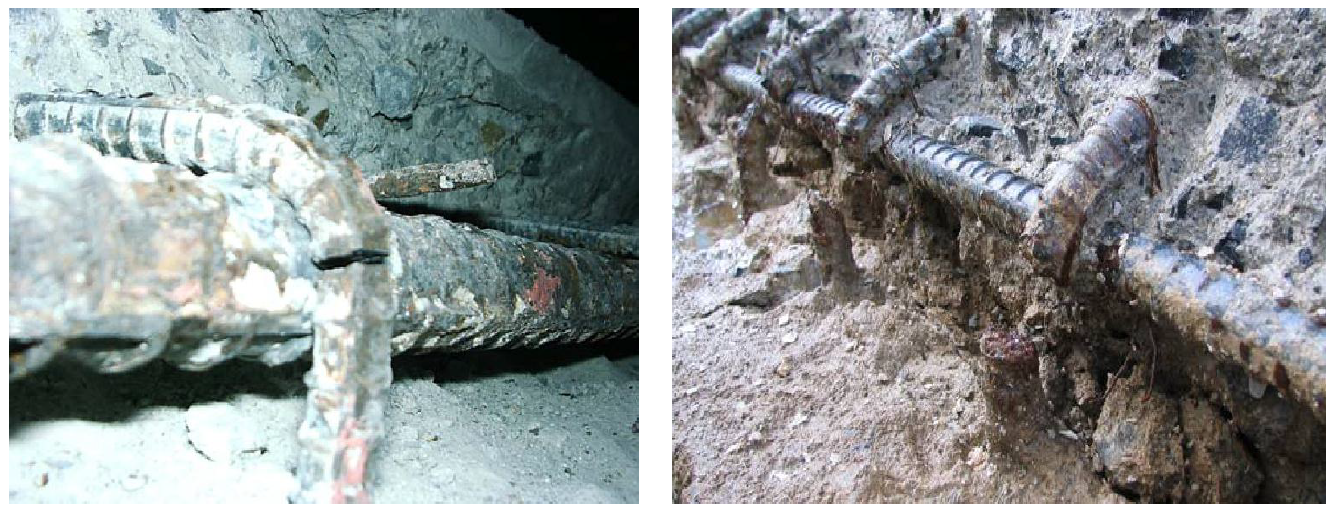
\includegraphics[width=.9\linewidth]{Files/Background/Miyagawa.png}
        \caption{Fractured stirrups in ASR-affected bridge piers in Japan [Miyagawa, et al. 2006, Torii, et al. 2008].}
        \label{fig:Miyagawa}
    \end{figure}

% DEF Examples

% ANUPUMN

Investigation done by A. Awasthi\cite{Awasthi} reveals large ettringite deposition in the damaged sleepers of Indian Railways.

    \begin{figure}[ht!]
        \centering
        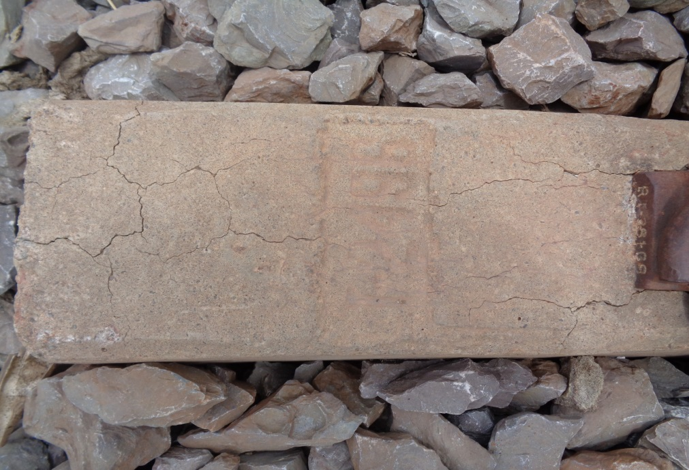
\includegraphics[width=.4\linewidth]{Files/Background/Anupam_1.png}
        \caption{Premature cracking of sleepers in Indian Railways[A. Awasthi, 2016].}
        \label{fig:Awasthi_1}
    \end{figure}

The problem of pre-mature cracking is investigated by collecting extensive samples from Indian Railways, studying the manufacturing processes, measured temperature inside concrete sleepers in the set up of a concrete sleeper plant, and analyzing samples using SEM (Scanning Electron Microscope), EDS (Energy-dispersive X-ray Spectroscopy) and XRF (X-ray Fluorescence).

In this research, EDS analysis confirmed the composition of DEF. Also, field measurement of temperature reveals that sleepers experiences high early age temperature (> 80$^\circ$C ), which is very critical for DEF problem to occur in future.

    \begin{figure}[ht!]
        \centering
        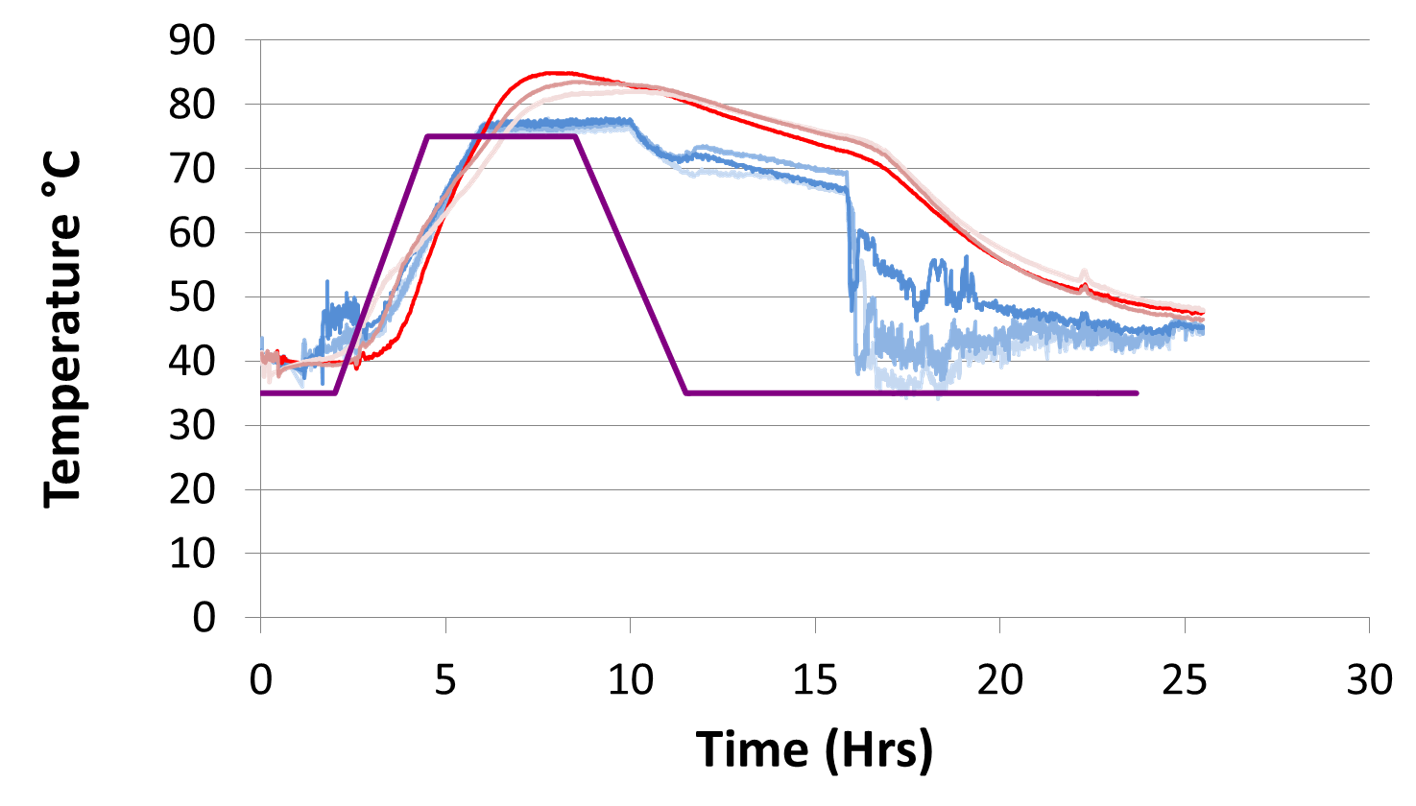
\includegraphics[width=.8\linewidth]{Files/Background/Anupam_2.png}
        \caption{Results of field measurement of temperature
 of sleepers during curing process in Indian Railways[A. Awasthi, 2016].}
        \label{fig:Awasthi_2}
    \end{figure}

Besides, in many cases, DEF has been accompanied by ASR, and may have been triggered in part by ASR (Folliard et al. 2006).

As a result of considerable research advances, ASR and DEF are now avoidable in new construction, but evaluating and managing the existing stock of structures damaged by these mechanisms remains a challenge.

Therefore, investigating how expansion from ASR and/or DEF affects on mechanical properties of concrete was the principal aim of this study.

In order to reach various expansion result, combinations such as different aggregate volume and different reactive aggregate were tried out by using concrete cube, 100x100x100 mm in size. By expanding the concrete model up to 1.3 percent, the relationship between mechanical properties losses and expansion can also be analyzed.

%*******10********20********30********40********50********60********70********80
\section{Literature Review}

\begin{itemize}

    \item
    \textbf{Evaluation of Concrete Structures Affected by Alkali-Silica Reaction and Delayed Ettringite Formation, E.R.Giannini, 2012}

    Four primary types of exposure site specimens were fabricated for this study, including Block, Unreinforced Slab-on grade, Reinforced Column, and Reinforced Bridge Deck.

    Aggregate in different level of reactivity are used for the exposure site specimens. Portland cements with high alkali contents were “boosted” with 50\% w/w NaOH solution to ensure that all specimens would undergo significant expansions within the time constraints of the project.

    \begin{figure}[ht!]
        \centering
        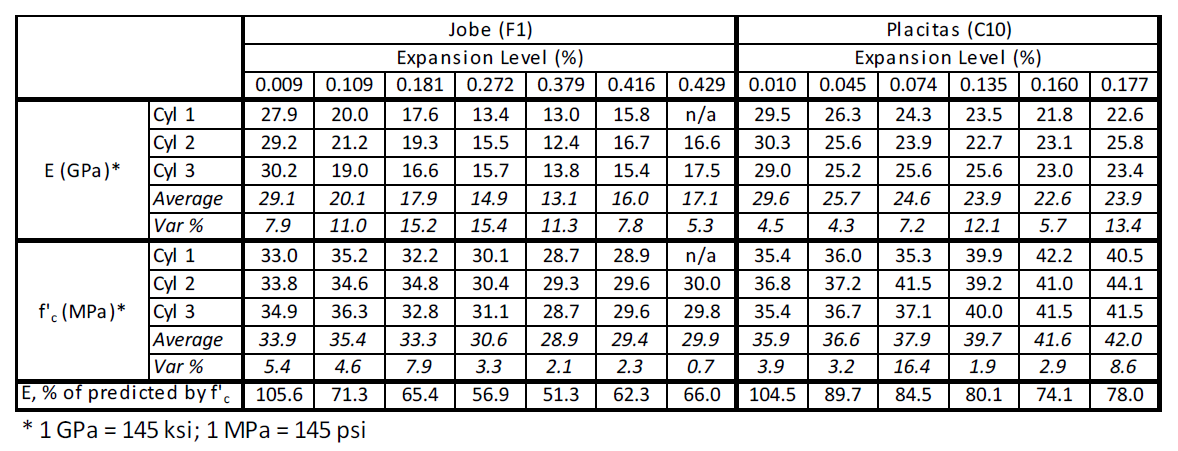
\includegraphics[width=.9\linewidth]{Files/Background/GIANNINI_ASR.png}
        \caption{Elastic modulus and compressive strength results for ASR cylinders. [E.R.Giannini, 2012].}
        \label{fig:GIANNINI_DEF}
    \end{figure}

    Additional procedures were involved to encourage the development of DEF. The cement and aggregates were heated in sealed buckets to 60$^\circ$C before mixing, while the mixing water was heated to 38$^\circ$C. The fresh concrete was quickly transported to a 60$^\circ$C chamber, placed and consolidated in foam-insulated wood forms. The forms were then covered in heavy blankets to minimize heat loss. After twelve hours, the heater for the chamber was turned off. The chamber was opened and the specimen allowed to slowly cool to ambient temperatures. Thermocouples recorded the temperature in the top, middle and base of the specimen. Peak curing temperature were well above the threshold necessary for the development of DEF.

    \begin{figure}[ht!]
        \centering
        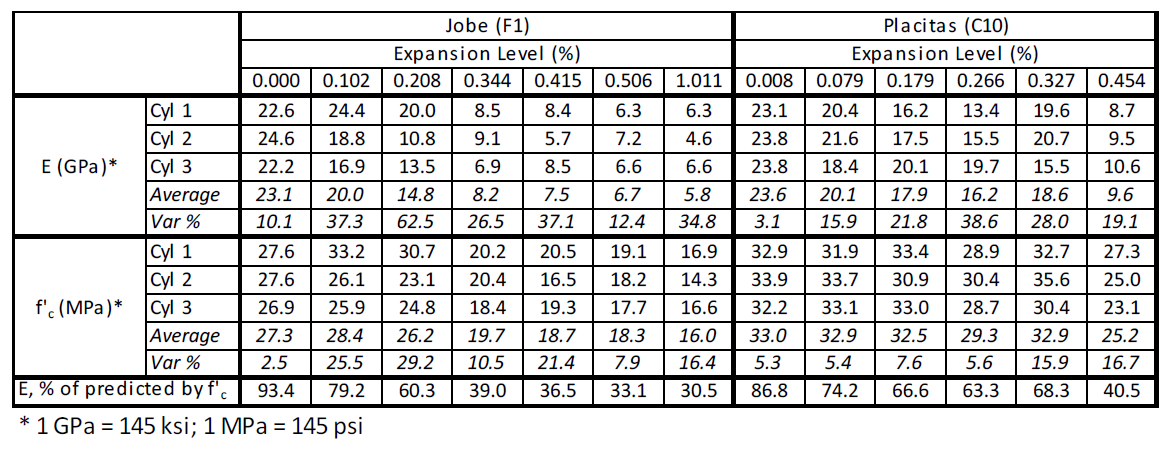
\includegraphics[width=.9\linewidth]{Files/Background/GIANNINI_DEF.png}
        \caption{Elastic modulus and compressive strength results for DEF cylinders. [E.R.Giannini, 2012].}
        \label{fig:GIANNINI_DEF}
    \end{figure}


    \item
    \textbf{The Effect Of Alkali Reactivity On the Mechanical Properties Of Concrete, T. Ahmed et al, 2013}

    In this study, T. Ahmed\cite{Ahmed} et al. used Thames Valley sand (in Mix A), fused silica (in Mix B) and slowly reactive aggregate (in Mix C) to investigate the effect of ASR expansion on compressive strength of concrete. Specimens in 100x100x100 size were cast and cured with respect to BS 1881 Part 122 [BS, 1881]. After casting and moulding, the cube specimens were cured for 28 days in water at $20^\circ$C and then the temperature was increased to $38^\circ$C to accelerate alkali-silica reaction. In this temperature, the specimens were stored at water tank until 12 months passed [Ahmed et al., 2003]. After 28-days curing at $20^\circ$C and storage at $38^\circ$C for 12 months, surface cracks are observed (Figure \ref{fig:T.Ahmed_crack}), and the expansion ratios along with compressive strength are given in Table \ref{table:Ahmed et al.}.

    \begin{figure}[ht!]
        \centering
        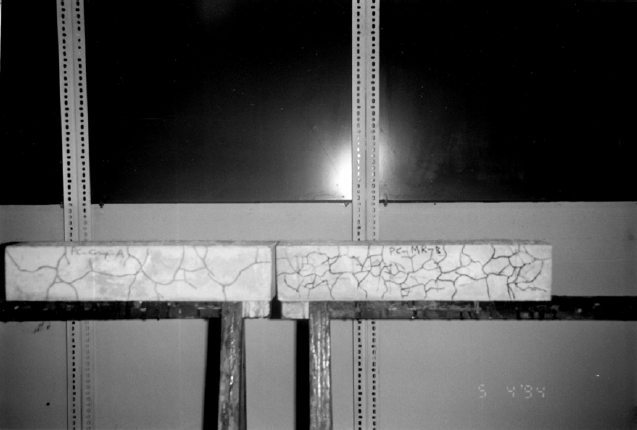
\includegraphics[width=.6\linewidth]{Files/Background/Ahmed_crack.png}
        \caption{Crack pattern of horizontally cast concrete prismcontaining Thames Valley sand (mix A) and 15\% fused silica (mix B) [Ahmed et al., 2003].}
        \label{fig:T.Ahmed_crack}
    \end{figure}

    \begin{table}[ht!]
        \centering
            \begin{tabular}{ |p{6cm}|p{1.5cm}|p{1.5cm}|p{1.5cm}| }
             \hline
             Mix &  A & B & C  \\ [0.5ex]
             \hline
             Expansion ratio (mm/mm) for 28-days curing at $20^\circ$C & -0.4 & 0.96 & 0.05 \\
             \hline
             Compressive Strength ($N/mm^2$) for 28-days curing at $20^\circ$C & 50.3 & 41.0 & 46.8 \\
             \hline
             Expansion ratio (mm/mm) for 12 months curing at $38^\circ$C & 4.3 & 16.86 & 1.27 \\
             \hline
             Compressive Strength ($N/mm^2$) for 12 months curing at $38^\circ$C & 57.0 & 26.5 & 65.3 \\ [0.5ex]
             \hline
            \end{tabular}
        \caption{Effect of ASR expansion on compressive strength of concrete [Ahmed et al., 2003].}
        \label{table:Ahmed et al.}
    \end{table}


    \item
    \textbf{Investigation of Premature Cracking of Sleepers in Indian Railways \& Evaluation of It's Residual Capacity, A. AWASTHI et al, 2016}

      In this study, A. Awasthi\cite{Awasthi} investigated the damaged premature cracking of sleepers, using the Scanning Electron Microscope (SEM) and Energy-Dispersive X-Ray Spectroscopy(EDS), confirmed the existing of DEF phenomenal in damaged concrete sleepers.

      \begin{figure}[ht!]
          \centering
          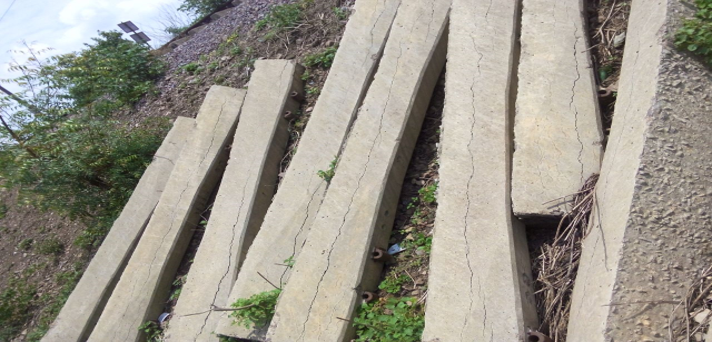
\includegraphics[width=.6\linewidth]{Files/Background/Anupam_3.png}
          \caption{Premature cracking of sleepers in Indian Railways[A. Awasthi, 2016].}
          \label{fig:Awasthi_3}
      \end{figure}

      The pre-heating process done on these concrete sleepers in order to achieve a high early strength (in case of Indian concrete sleepers the steam curing temperature is 75 $\circ$C) and subsequent exposure to moisture during service lead the formation of delayed ettringite. Temperature measurement was performed in concrete sleeper plant in India both inside and outside of concrete reveals that temperature inside the concrete sleeper is much higher than the outer part, the high temperature over 80$\circ$C is a very critical factor for the occurrence of damage due to DEF.

      \begin{figure}[ht!]
          \centering
          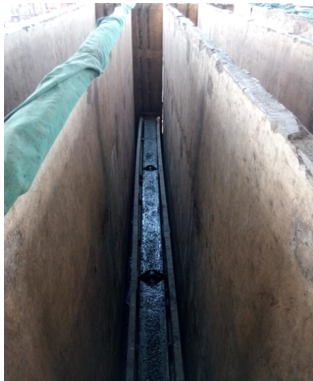
\includegraphics[width=.4\linewidth]{Files/Background/Anupam_4.png}
          \caption{Temperature measurement for pre-heating process of Indian Concrete Sleeper [A. Awasthi, 2016].}
          \label{fig:Awasthi_4}
      \end{figure}

    \item
    \textbf{Mesoscopic analysis of different expansion causes in concrete by 3D Rigid Body Spring Model, L. EDDY, A. AWASTHI, K, MATSUMOTO, K. NAGAI, and S.ASAMOTO, 2017}

    This study done by L. EDDY et al.\cite{EDDY} developed the 3 dimensional numerical discrete analysis model using RBSM for mesoscopic analysis of different expansion, including both ASR expansion and DEF expansion.


    \begin{figure}[ht!]
    \centering
    \begin{subfigure}{.5\textwidth}
      \centering
      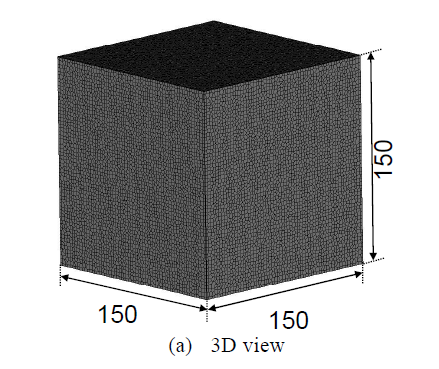
\includegraphics[width=.9\linewidth]{Files/Background/EDDY_model_1.png}
    \end{subfigure}%
    \begin{subfigure}{.5\textwidth}
      \centering
      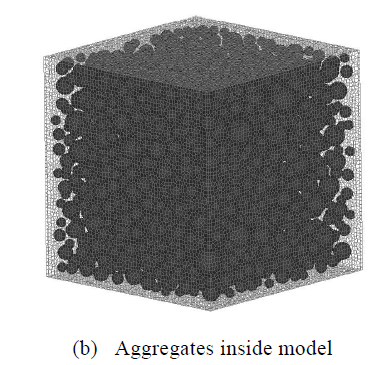
\includegraphics[width=.75\linewidth]{Files/Background/EDDY_model_2.png}
    \end{subfigure}
    \caption{3D Concrete Model (units: mm) [L.EDDY et al.]}
    \label{fig:EDDY_model}
    \end{figure}

    Fig \ref{fig:EDDY_model} shows the analyzed numerical model. The size of the model is 150x150x150 mm. Aggregate volume is 26\% in this research.

    \begin{figure}[ht!]
        \centering
        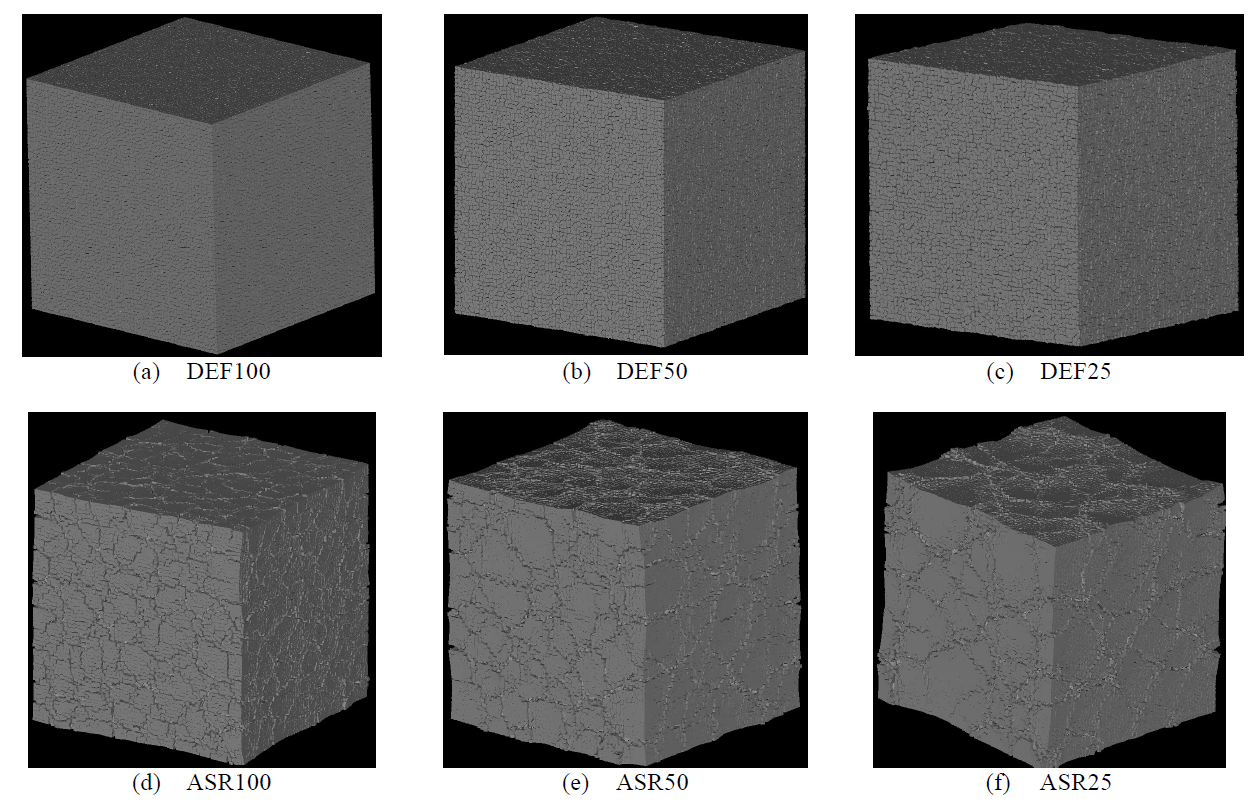
\includegraphics[width=.9\linewidth]{Files/Background/EDDY.png}
        \caption{Surface Cracks (Deformation x 10) [L.EDDY et al.]}
        \label{fig:EDDY}
    \end{figure}

    In the ASR-type cases, the expansion strain is applied at the mortar-aggregate interfaces to reflect the expansion due to the alkali silicate gel product formed in the aggregates.

    Three numerical models, named by ASR100, ASR50, and ASR25 are considered in ASR simulations. ASR100 means that all the mortar-aggregate interfaces expand. ASR50 means that 50\% of all springs between mortar-aggregate interfaces (randomly selected) expand. While ASR25 means that 25\% of all springs between mortar-aggregate interfaces (randomly selected) expand.

    Stress in the aggregates and mortar decreases because localized cracks in the mortar open. With less percentage of locations of the mortar-aggregate interface expansion, cracks become more localized. These localized cracks int he mortar and the expansion at the mortar-aggregate interfaces are connected to form the map cracks occur in the concrete.

    In the cases for DEF-type, the expansion strain is applied in the mortar to represent the paste expansion. However, based on the simulation results, DEF-type cases do not match well with the typical map cracking pattern observed in the real concrete.

    Meanwhile, three numerical models, named by DEF100, DEF50, DEF25 are considered in this DEF simulations. DEF100 means that all springs between mortar elements expand. DEF50 means that 50\% of all springs between mortar elements (randomly selected) expand. While DEF25 means that 25\% of all springs between mortar elements (randomly selected) expand.

    E. Liyanto and team proposed that simple model as uniform expansion of paste takes place in DEF could not reproduce the typical cracking pattern of DEF. In order to simulate the DEF appropriately, the simple model in this study needs to be improved because there might be more complex phenomenon occurred.

\end{itemize}

%*******10********20********30********40********50********60********70********80

\section{Deformation Mechanism for ASR and DEF}

ASR and DEF, though produce similar visual indications (charcteristic map surface cracking), the mechanism of each is different. A short discussion of the two mechanisms is provided below.

\subsection{Alkali-Silica Reaction (ASR)}

Firstly identified by Stanton\cite{Stanton} over 70 years ago, ASR is a important reason of concrete deterioration. Since that time, ASR has been identified as a cause of deterioration of numerous concrete structures.

%Stanton, T. E. "Expansion of Concrete through Reaction between Cement and Aggregate." Publications of the American Society of Civil Engineers 66 (1940): 1781-1811.

Alkali silica reaction (ASR) is a deleterious chemical reaction, between some siliceous minerals in the aggregate and the alkalinity of the concrete.

As the result, a hydrophilic gel named ASR gel is formated and swells in the presence of moisture, causing the expansion of concrete. Figure \ref{ASR_mechanism} by Kreitman, K\cite{Kreitman} illustrates the mechanism of ASR.

%Kreitman, K. "Nondestructive Evaluation of Reinforced Concrete Structures Affected by Alkali-Silica Reaction and Delayed Ettringite Formation." MS Thesis, The University of Texas at Austin, Austin, Texas, 2011.

\begin{figure}[ht]
\centering
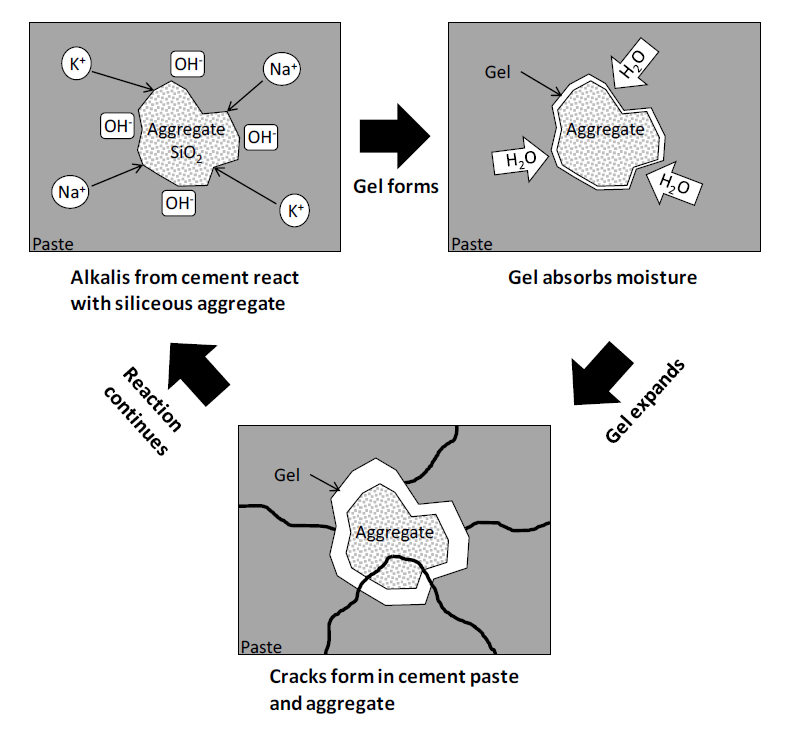
\includegraphics[width=.8\linewidth]{Reference/Kreitman.png}
  \caption{Mechanism of alkali-silica reaction [Kreitman 2011]}
  \label{ASR_mechanism}
\end{figure}

According to G.K. Glass\cite{Glass} in book Comprehensive Structural Integrity, 2003, factors which control the reaction rate and degree of expansion include the alkali content, the quantity of reactive aggregate and its particle size, the moisture content of the concrete and moisture content variations, temperature and the permeability of the concrete.

%G.K. Glass, in Comprehensive Structural Integrity, 2003

Although countermesures has yielded considerable success in minimize the risk of expansive ASR in new construction, the capability of ASR damaged concrete remains a major topic of ongoing research.

%%%%%%%%%%%%%%%%%%%%%%%%%%%%%%%%%%%%%%%%%%%%%%%%%%%%
\subsection{Delayed Ettringite Formation (DEF)}

Delayed Ettringite Formation (DEF) is a form of internal sulfate attack in concrete, driven by high curing temperatures and unfavorable cement chemistry (Kelham 1996\cite{Kelham}). Many laboratory studies have confirmed that 70$^\circ$C is the critical curing temperature for expansion due to DEF(H.F.W. Taylor et al., 2000\cite{Taylor}).

%Kelham, S. "The Effect of Cement Composition and Fineness on Expansion Associated with Delayed Ettringite Formation." Cement & Concrete Composites 18 (1996): 171-179.

%H.F.W Taylor, C. Famy, K.L. Scrivener. "Review: Delayed Ettringite Formation", Cement and Concrete Research 31(2001) 683-693

The hydration of cement and formation of C-S-H is greatly accelerated as curing temperature increases (Folliard, et al. 2006\cite{Folliard}). The rapidly growing “outer” C-S-H is different than that which forms at lower temperatures and traps dissolved sulfates before they can react to form ettringite, another normal product of cement hydration. With sustained temperatures above 70$^\circ$C, ettringite becomes thermodynamically unstable and either does not form or returns to solution.

%Folliard, K. J., et al. Preventing ASR/DEF In New Concrete: Final Report. Austin: Center for Transportation Research, 2006.

 Based on thermodynamics and X-ray diffraction observations, other hydration products, stable at high temperatures, such as calcium monosulfoaluminate (monosulfate) and hydrogarnet form instead from the decomposing ettringite and remaining aluminates, ferrites and sulfates in solution (Ramlochan 2003\cite{Ramlochan}).

 %Ramlochan, T. "The Effects of Pozzolans and Slag on the Expansion of Mortars and Concrete Cured at Elevated Temperature." PhD Thesis, Toronto: University of Toronto, 2003.

Once temperatures return to normal level, thermodynamics assist the formation of ettringite. Sulfates may be released from the C-S-H, then react with water and monosulfate, form ettringite, and lead to deleterious expansion and cracking of the concrete (Folliard et al, 2006\cite{Folliard}). A illustration of the mechanism of DEF is shown in Figure \ref{DEF_mechanism}.

 \begin{figure}[ht]
 \centering
 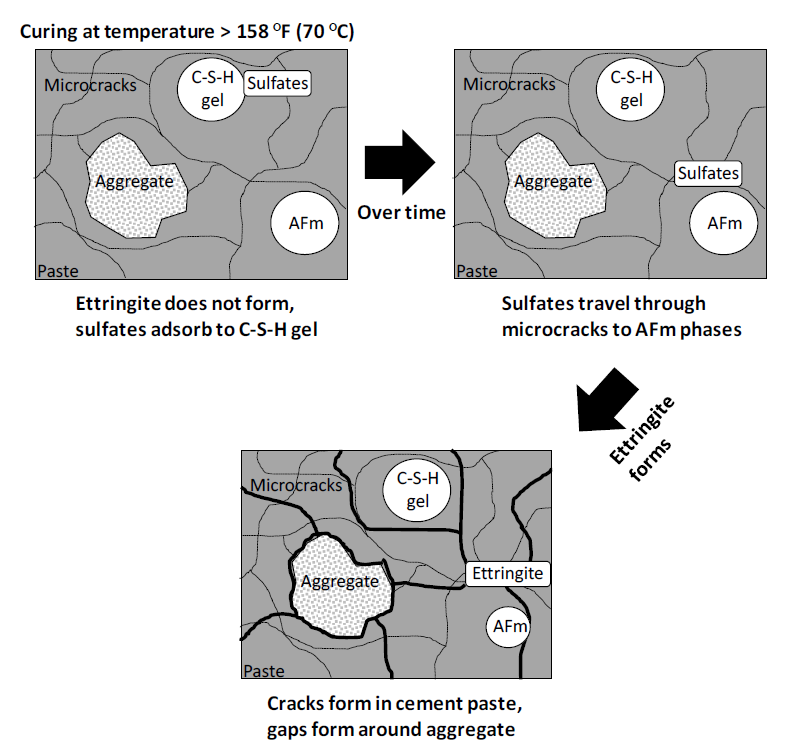
\includegraphics[width=.8\linewidth]{Reference/Kreitman2.png}
   \caption{Mechanism of delayed ettringite formation [Kreitman 2011]}
   \label{DEF_mechanism}
 \end{figure}


%*******10********20********30********40********50********60********70********80
\section{Research Objective}

The final goal of this research is to develop the simulation system which has ability for revealing the residual capacity of ASR and/or DEF expansion deteriorated structure.

Considering our research group’s simulation systems, 3D RBSM was conducted for the quantities evaluation of concrete behavior by directly modeling the shape of aggregates.

Considering the previous study about the expansion of concrete structure in literature review, in order to achieve the final goal, the following objectives are set as the research’s goal:

\begin{itemize}

    \item Develop the simulation of concrete damage from the ASR expansion. Once the ASR expanse occurred, the initial strain will be given at the interfaces between reactive aggregate and mortar. As a result, increasing of tensile stress of concrete around the reactive aggregate will lead to the cracking.

    \item Develop the simulation of concrete damage from the DEF expansion. Once the DEF expanse occurred, the initial strain will be given at the interfaces between mortar elements. As a result, increasing of tensile stress of inside concrete paste will lead to the cracking.

    \item Develop the uni-axial compression test for represent the residual mechanical properties of expanded concrete models. Concrete's behavior under loading and its proprieties such as compressive strength and elastic modulus in macro scale will be obtained.

\end{itemize}



%*******10********20********30********40********50********60********70********80
\section{Organization of Contents}

The development of simulation and mechanical properties test in ASR and/or DEF expanded concrete will be explained in this thesis following structure as shown below:

\begin{itemize}

    \item Chapter 1 : Introduction.

    In this chapter, detailed about research background, statement of problem and objective are explained. Some literature reviews that related to the developing.

    \item Chapter 2 : Simulation model.

    In this chapter, the method in development of each numerical simulation model, related literature review of previous studies, will be described. The development of constitutive model for the expansion will be explained. The method for given expansive strain for simulating the same concrete damage will be explain step by step. The theoretical formulation related in numerical analysis of expanding behaviour are also described in this section.

    \item Chapter 3: Simulation of Cracking Pattern Of ASR and DEF Expanded Concrete.

    In this chapter, details about the surface and cross section cracking pattern results caused by ASR and/or DEF expansion are summarized, comparing between different cases and also with the experimental results.

    \item Chapter 4: Simulation of Residual Mechanical Capabilities Of ASR and DEF Expanded Concrete.

    In this chapter, details about the residual mechanical properties, including residual compressive strength and residual elastic modulus, are summarized. The relationships between residual capacity and expansion behavior due to different expansion causes are also discussed.

    \item Chapter 5: Conclusions

    In this final chapter, several remarks about the capability of ASR and/or DEF expansion simulation are emphasized. Also, some commentaries for further project or improvement are proposed.


\end{itemize}
